

\begin{frame}[t,allowframebreaks]{
    Trade off between bias and variance -}

The \index{bias}\gls{bias} and the \index{variance}\gls{variance}
are {\bf different sources of error} in an estimator.\\
\vspace{0.2cm}

The {\bf mean squared error (MSE) or our estimate},
expressing the overall expected (squared) deviation, 
is given by:
\begin{equation}
    MSE = 
      \mathbb{E}\Big( 
        (\vect{\hat{\theta}}_{\mathbb{X}_{m}} - \vect{\theta})^2        
       \Big) =
       bias(\vect{\hat{\theta}}_{\mathbb{X}_{m}})^2 +
       var(\vect{\hat{\theta}}_{\mathbb{X}_{m}})
    \label{eq:mse_estimation}
\end{equation}\\

\vspace{0.2cm}

{\bf Desirable estimators have small MSE.}
\begin{itemize}
    \item
    Between estimators with more \gls{bias} and estimators 
\end{itemize}

\framebreak

%
%

The relationship between \gls{bias} and \gls{variance} is
linked to the concept of a 
\gls{ml} model \index{capacity}\gls{capacity}
and to the pathologies of 
\index{underfitting}\gls{underfitting} and
\index{overfitting}\gls{overfitting}.

\begin{center}
    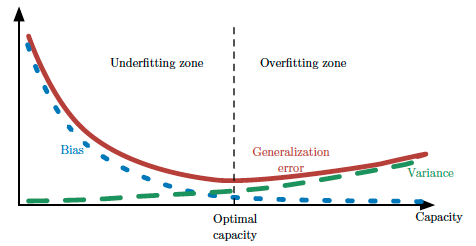
\includegraphics[width=0.80\textwidth]
        {./images/training_issues/goodfellow17_bias_variance_tradeoff_1.png}\\
    {\tiny 
        Illustrating the trade off between bias and variance.
        As the capacity increases, bias decreases and variance increases
        yielding a U-shaped curve from where an optimal capacity can be deduced.\\
        \color{col:attribution} 
        Schematic reproduced from p. 127 of \cite{Goodfellow:2017MITDL}.\\
    }
\end{center}        

\end{frame}
